We started with a two body system and did some calculations with both Euler's method and the Velocity Verlet method. Thereafter we added another planet, Jupiter, and saw how this affected the system. At last we added all the planets using initial conditions from NASA \cite{nasa} [FIX THIS LATER]. Our solar system thus far had been non-relativistic, only  Newtonian forces was taken into consideration. To investigate how relativistic forces affect the solar system, we looked at the perihelion precession of Mercury.

\subsection{Two body system}

We started out with a two body system consisting of the sun and the earth. The origin of the system was the sun's position at time = 0. We wanted to find out what initial velocity the earth needed to have, for the orbit of the earth to be circular. The result can be found in Figure \ref{fig:circular_orbit}.

\begin{figure}[H]
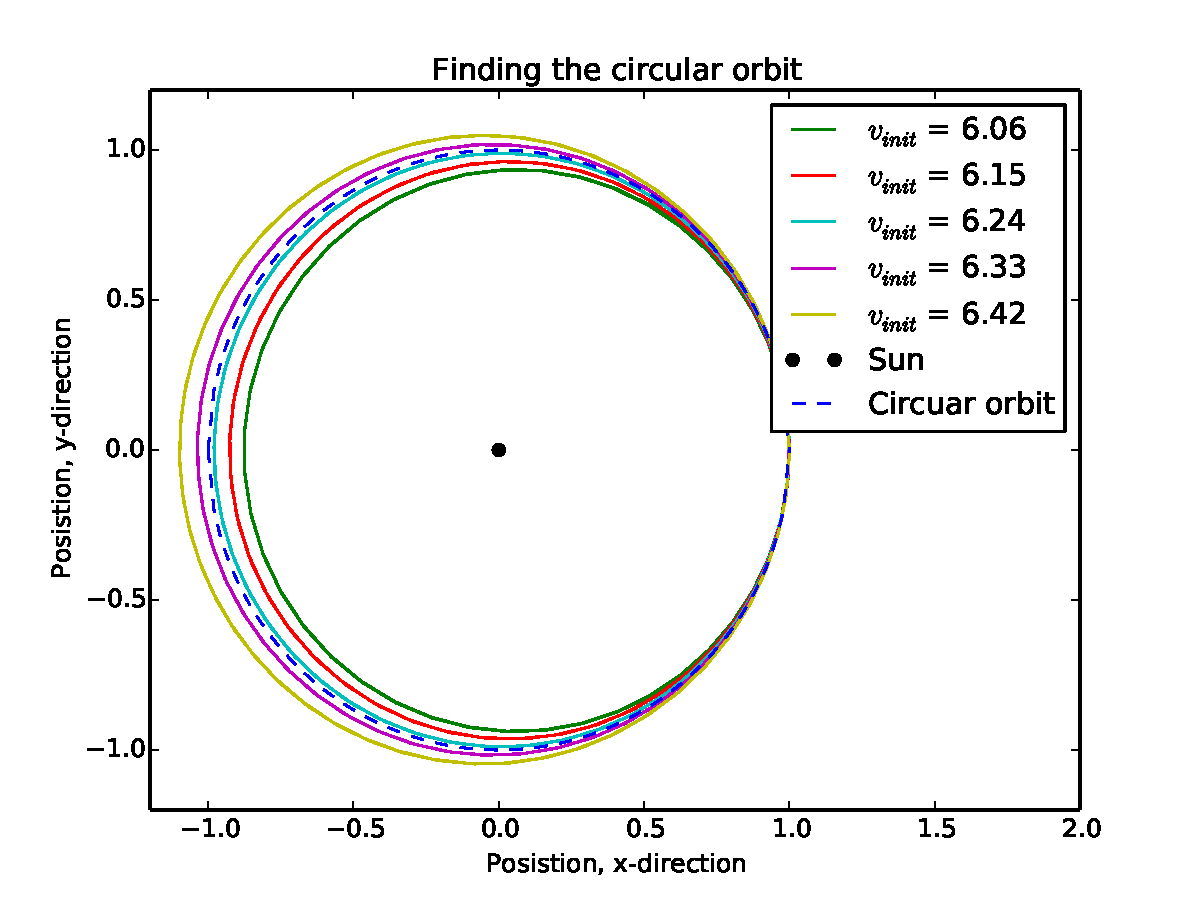
\includegraphics[width=0.9\linewidth]{../results/plots/circular_orbit.pdf}\caption{This is a plot of the orbit with different initial velocities. The circular orbit has a velocity between 6.24 and 6.33. $2 \pi \approx 6.28$ is the initial velocity that gives a circular orbit \ref.}\label{fig:circular_orbit}
\end{figure}

As mentioned in the method part of this report, we used two different methods to solve the differential equations, to simulate the motion, Euler's method and the Velocity Verlet method. We started out by plotting the circular motion of the earth with different time steps (see Figure \ref{fig:timesteps-euler} and \ref{fig:timesteps-verlet})to be able to evaluate the two methods.
	
\begin{figure}[H]
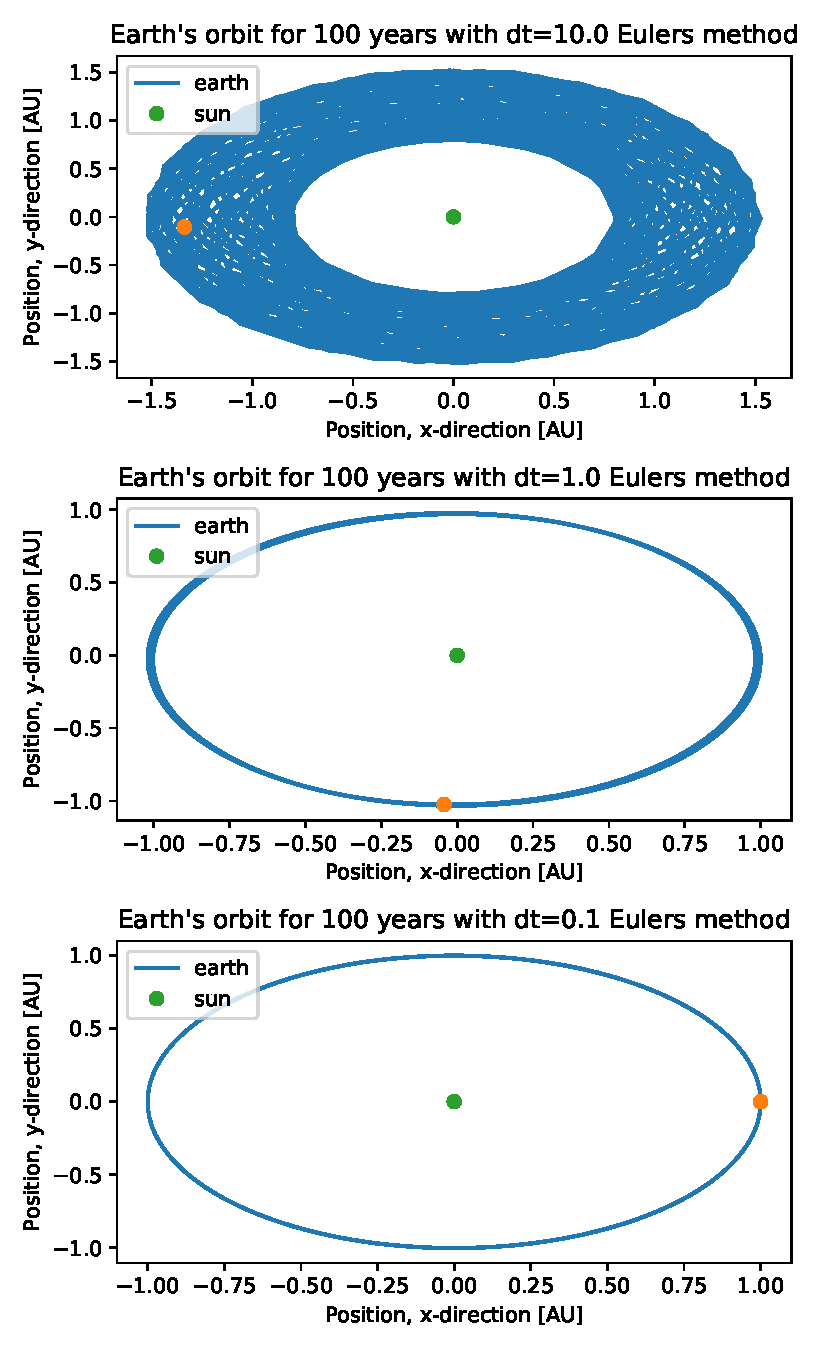
\includegraphics[width=0.9\linewidth]{../results/plots/different_timesteps_Eulers_method.pdf}\caption{This is a plot of the earth's orbit for 100 years using Euler's method, with different timesteps.}\label{fig:timesteps-euler}
\end{figure}		

After 
\begin{figure}[H]
	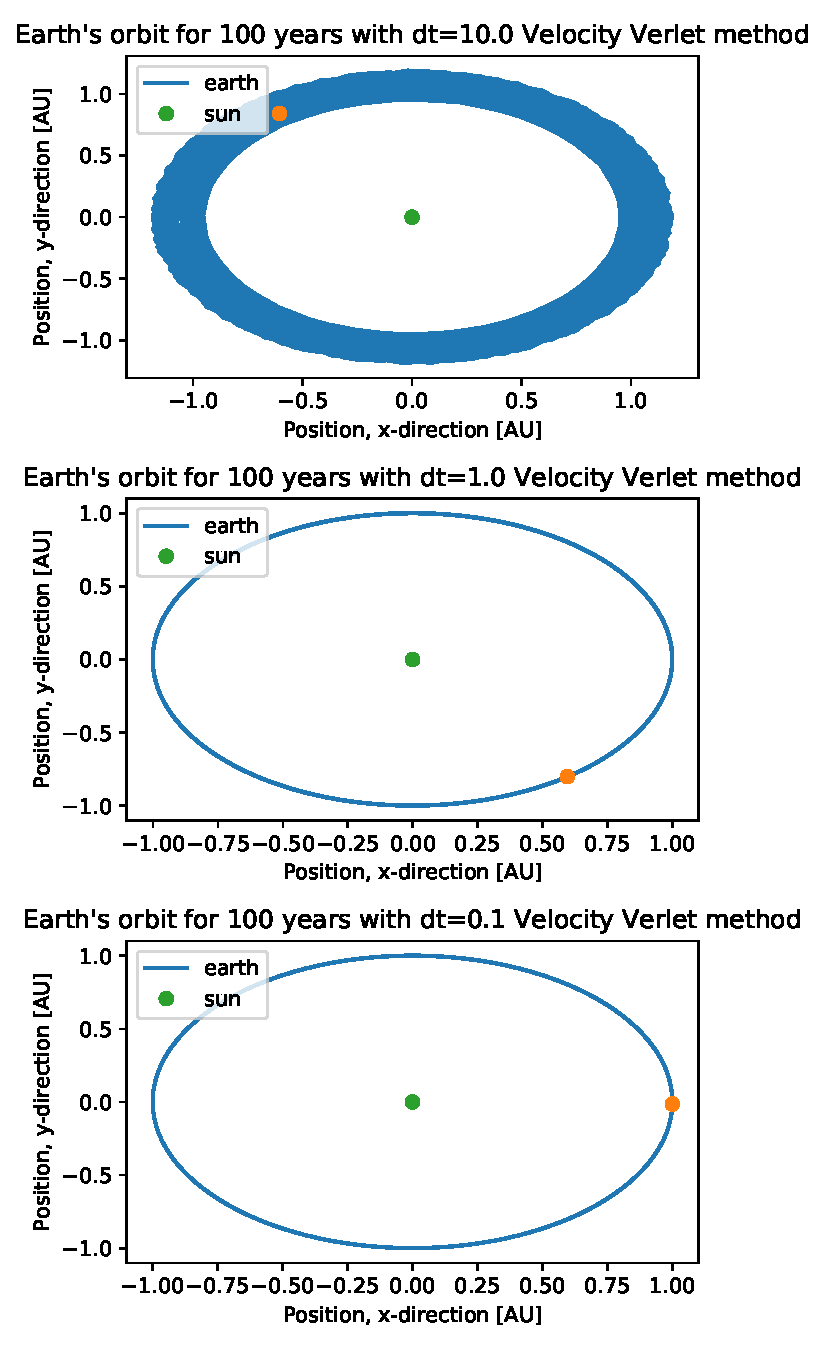
\includegraphics[width=0.9\linewidth]{../results/plots/different_timesteps_Velocity_Verlet_method.pdf}\caption{This is a plot of the earth's orbit for 100 years using the Velocity Verlet method, with different timesteps.}\label{fig:timesteps-verlet}
\end{figure}		

Another way to compare two methods are looking at the CPU time. In Table \ref{tab:CPUtime} the CPU time for the two method are listed. We can see that the difference between them are small, but the velocity Verlet algorithm is slower than the Euler method. 


\begin{table}[H]\caption{Comparison of CPU time of Euler's method and the Velocity Verlet method (VV). Calculations were performed with 1000 time steps per year. As the CPU-time also calculate the time spent on updating energies and calling several functions, one will not be able to read out the CPU time of the euler/velocity verlet loop alone.}\label{tab:CPUtime}
	\begin{tabular}[width=\linewidth]{cccc}
		Years &\small{ time Euler  } & \small{time VVerlet} & \small{$\Delta time $} \\
		& (ms)&(ms) &(ms)\\ \hline 
		    
		100 & 88.728 & 93.646 & 4.912 \\
		1000 & 812.486 & 852.949   &40.46\\	
		10000 & 	8145.7  & 8504.06   &358.36
	\end{tabular}
\end{table}

%\begin{figure}[H]
%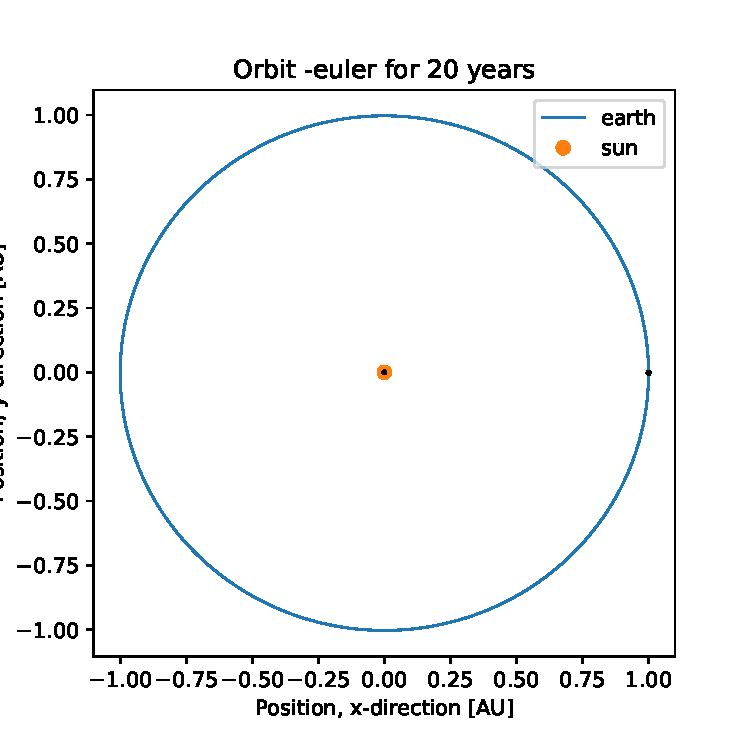
\includegraphics[width=0.9\linewidth]{../results/plots/plotof-earthsun-euler.pdf}\caption{This is a plot of the earth's orbit for 100 years using Euler's method, with 1000 timesteps per year, to simulate the motion.}\label{fig:earth-sun-euler}
%\end{figure}		
%	
%\begin{figure}[H]
%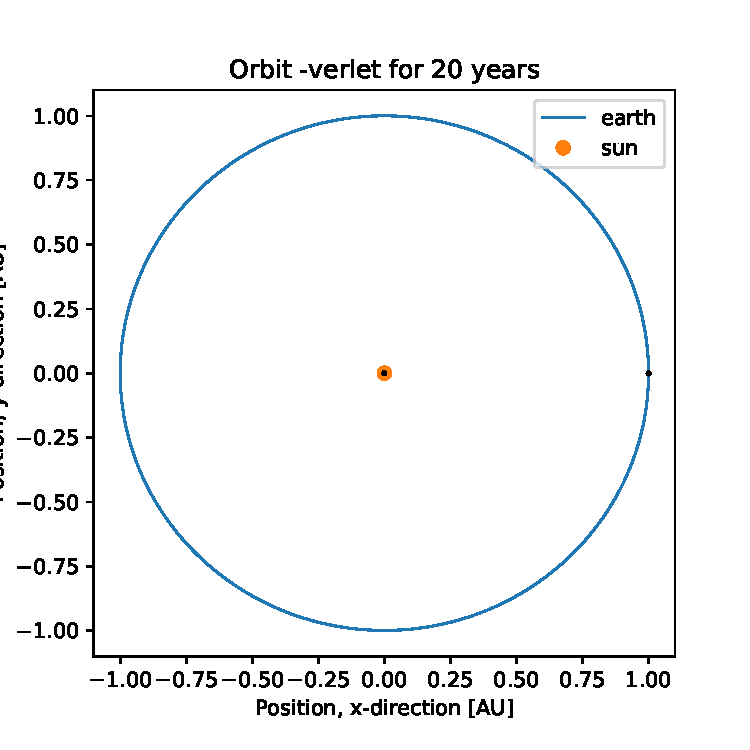
\includegraphics[width=0.9\linewidth]{../results/plots/plotof-earthsun-verlet.pdf}\caption{This is a plot of the earth's orbit for 100 years using the velocity Verlet method, with 1000 timesteps per year, to simulate the motion.}\label{fig:earth-sun-verlet}
%\end{figure}	

\subsection{Conservation}

First we checked if the angular momentum of the two body system was conserved. Figure \ref{fig:angluarmomentum-euler} and \ref{fig:angularmomentum-verlet} shows the results. The angular momentum is not totally conserved. The values are oscillating and there is an increase in the angular momentum when we use the Velocity Verlet method and a decrease when we use Euler's method. The scale of the change though is on the level of $10^{-10}$ for Euler's and $10^{-11}$ for Velocity Verlet. That is small compared to the whole value that are on the $10^{-5}$.

\begin{figure}[H]
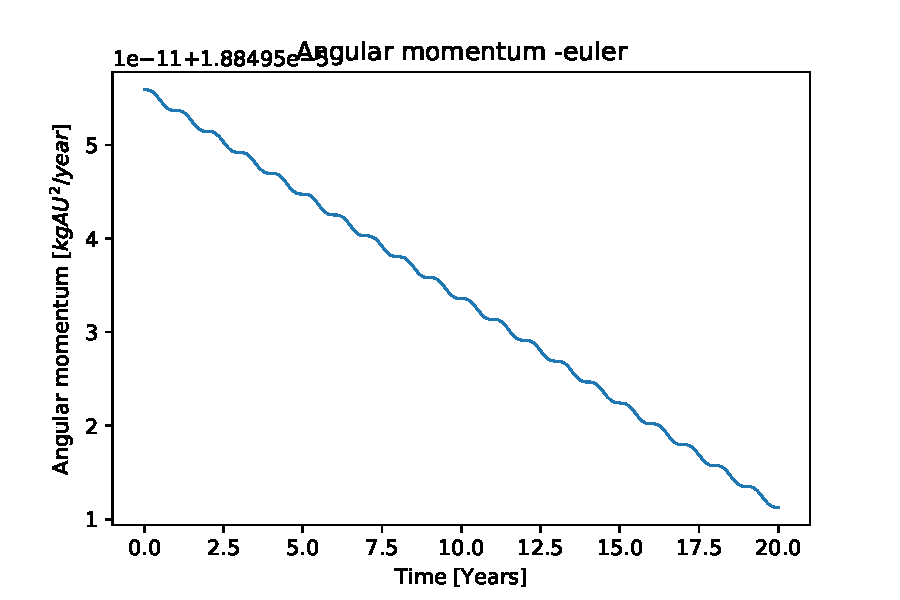
\includegraphics[width=0.9\linewidth]{../results/plots/angularmomentum-euler.pdf}\caption{This is a plot of the angular momentum of the sun-earth system for 20 years using Euler's method, with 1000 timesteps per year. Notice that the scale of the axis is a sum.}\label{fig:angluarmomentum-euler}
\end{figure}	

\begin{figure}[H]
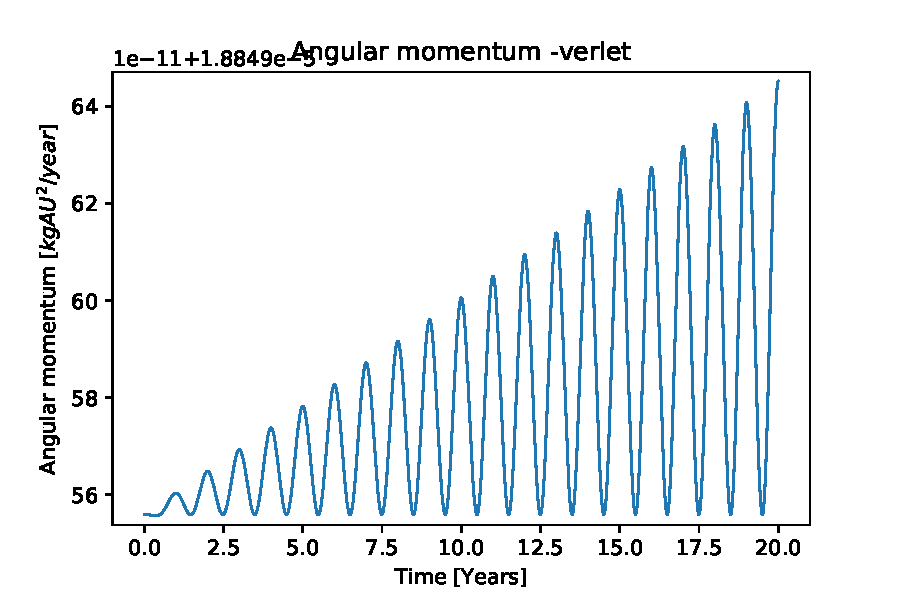
\includegraphics[width=0.9\linewidth]{../results/plots/angularmomentum-verlet.pdf}\caption{This is a plot of the angular momentum of the sun-earth system for 20 years using the velocity Verlet method, with 1000 timesteps per year. Notice that the scale of the axis is a sum.}\label{fig:angularmomentum-verlet}
\end{figure}	

The other important parameter that needs to be conserved is the energy. Figure \ref{fig:totalenergy-euler} and \ref{fig:totalenergy-verlet} shows the energy development of the two methods, Euler's and Velocity Verlet respectively. The total energy is oscillating like the angular momentum and slightly changing, but the scales are small here two. Table \ref{tab:energy_oscillations} lists the difference in the oscillation amplitudes of the two methods. 

\begin{figure}[H]
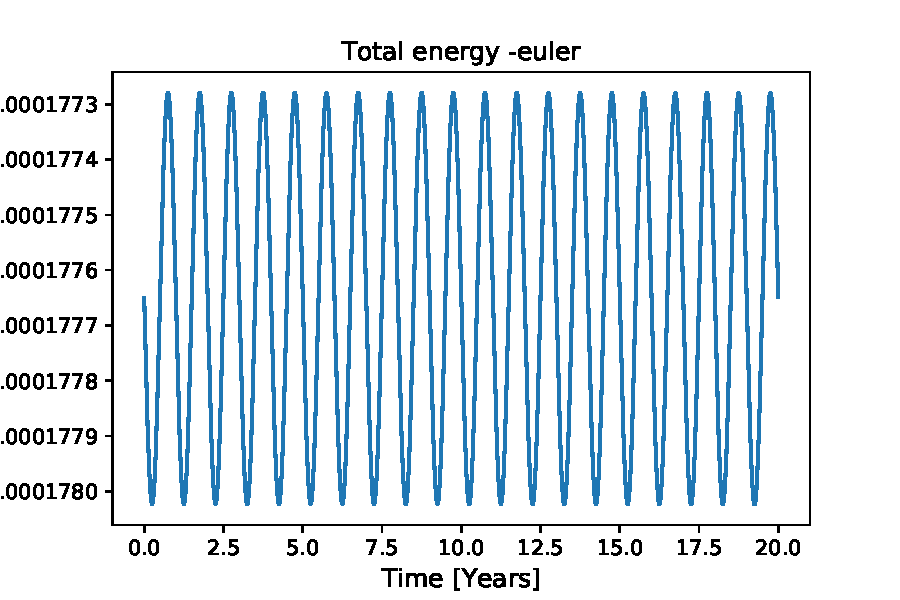
\includegraphics[width=0.9\linewidth]{../results/plots/totalenergy-euler.pdf}\caption{This is a plot of the total energy of the sun-earth system for 20 years using Euler's method, with 1000 timesteps per year.}\label{fig:totalenergy-euler}
\end{figure}	

\begin{figure}[H]
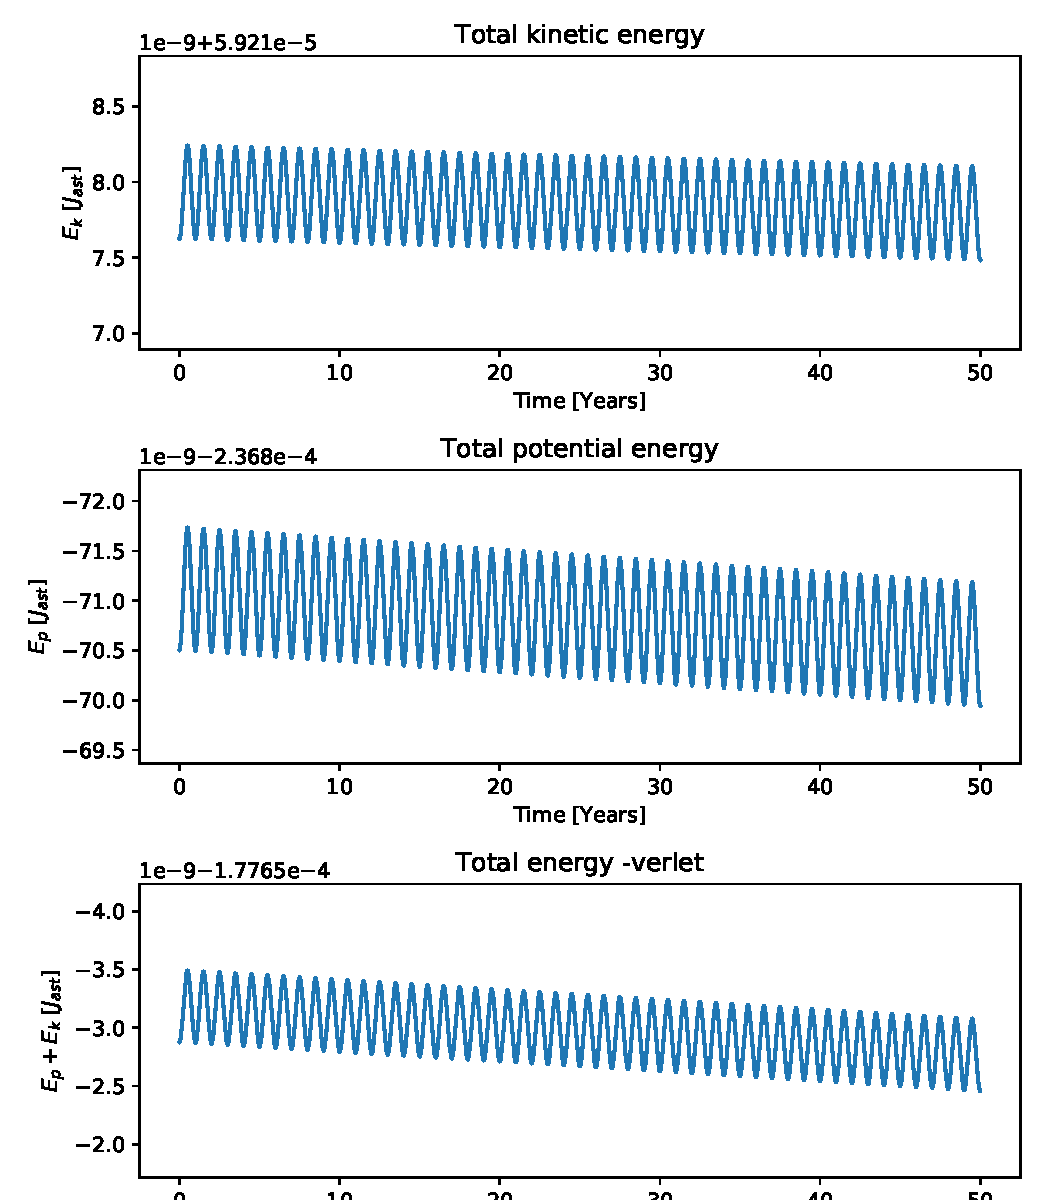
\includegraphics[width=0.9\linewidth]{../results/plots/totalenergy-verlet.pdf}\caption{This is a plot of the total energy of the sun-earth system for 20 years using the velocity Verlet method, with 1000 timesteps per year.}\label{fig:totalenergy-verlet}
\end{figure}

\begin{table}[H]\caption{This is a table that list how the energy oscillates in the two different method. These are only approximate values that are read form the plots of the energies (Figure \ref{fig:totalenergy-euler} and \ref{fig:totalenergy-verlet}). Plot of kinetic and potential energies can be found in the appendix.} \label{tab:energy_oscillations}
\begin{tabular}{lcc}
\small{Oscillation of:} & \small{Euler's:} & \small{Velocity Verlet:}\\ \hline
\small{Kinetic energy} [ $J_{ast}$]: & $0.8\cdot10^{-6}$ & $1.5 \cdot 10^{-9}$  \\
\small{Potential energy} [ $J_{ast}$]: & $1.5\cdot 10^{-6}$ & $3\cdot10^{-9}$  \\
\small{Total energy} [ $J_{ast}$]:  & $ 5 \cdot 10^{-6}$ & $2\cdot10^{-9}$ \\
\end{tabular}
\end{table}

\subsection{Checking gravitational forces}

To check the gravitational force working on the earth from the sun in our two body system, we started by testing earth's necessary initial velocity to escape the sun, the escape velocity. Figure \ref{fig:escape_velocity_exact} shows the plot of the exact escape velocity and Figure \ref{fig:escape_velocity_near_exact} show some of the velocities near the exact escape velocity.

\begin{figure}[H]
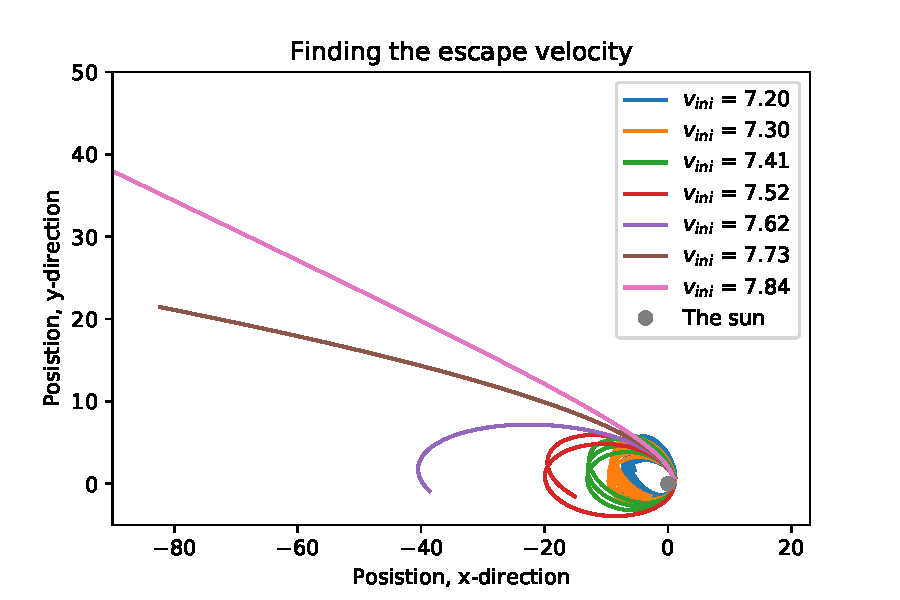
\includegraphics[width=0.9\linewidth]{../results/plots/escape_velocity.pdf}\caption{This is a plot of the sun-earth system for the exact initial velocity that allows the earth to escape the sun.}\label{fig:escape_velocity_exact}
\end{figure}

\begin{figure}[H]
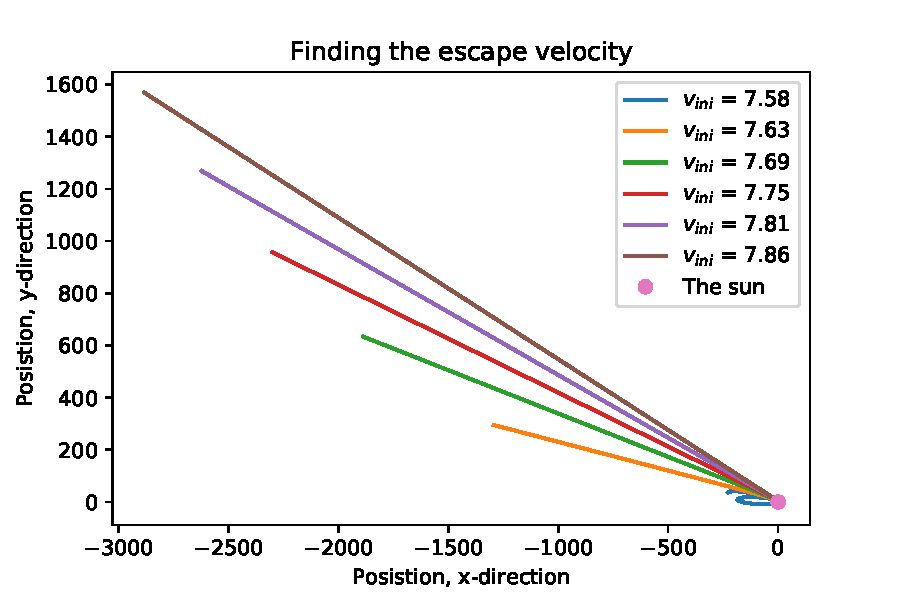
\includegraphics[width=0.9\linewidth]{../results/plots/escape_velocity_closeto_exact.pdf}\caption{This is a plot of the sun-earth system for different initial velocities. The plot shows initial velocities near the exact escapevelocity, $2\pi\sqrt{2} \approx 8.88 $. }\label{fig:escape_velocity_near_exact}
\end{figure}

Next we wanted to see what happened if we changed the gravitational force. The gravitational force is given by $ F = \frac{GM_EM_S}{r^\beta}$ where $\beta$ is 2. In Figure \ref{fig:different_gravitation} we plotted the motion of the earth with different $\beta$ between 2 and 3.

\begin{figure}[H]
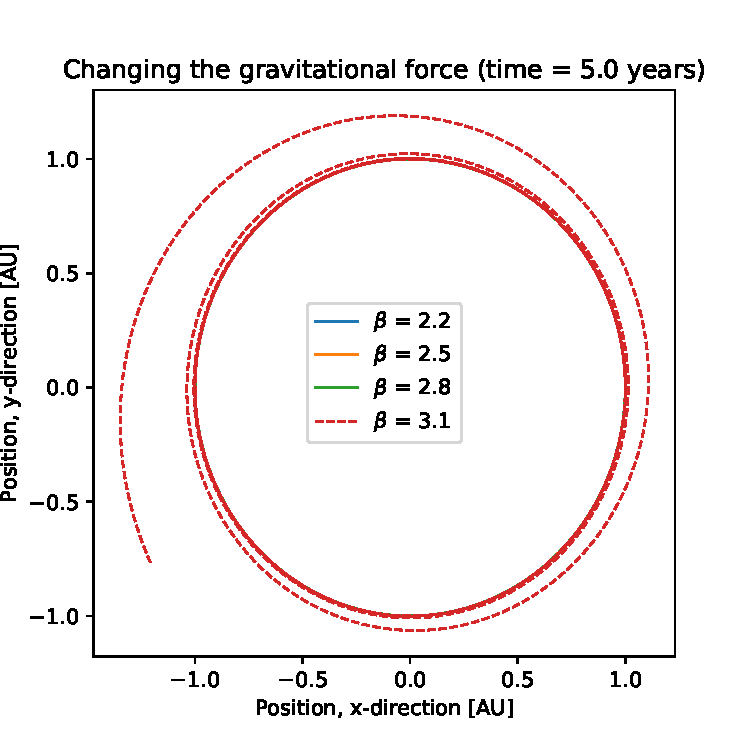
\includegraphics[width=0.9\linewidth]{../results/plots/diffenrent_gravitation.pdf}\caption{This is a plot of the sun-earth system for different gravitational forces. The gravitational force is given by $ F = \frac{-GM_EM_S}{r^\beta}$ and in the plot $\beta$ is changed from it's normal value $\beta = 2$ to $\beta = 3.1$.}\label{fig:different_gravitation}
\end{figure}

\subsection{Three body system}

Next we added a planet, Jupiter, to our system and got a three body problem. Figure \ref{fig:three_body_sun_origin} shows the motion of the planets.

\begin{figure}[H]
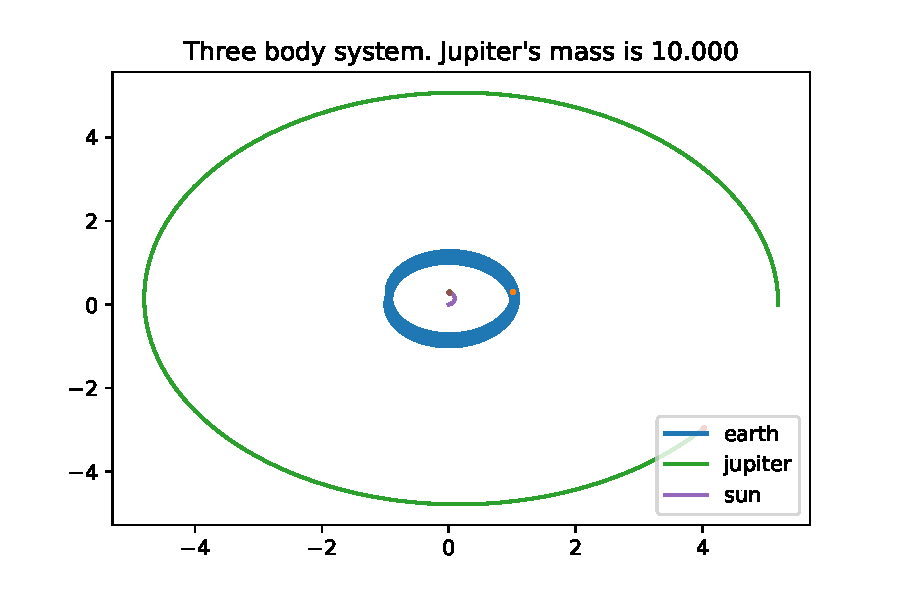
\includegraphics[width=0.9\linewidth]{../results/plots/Jupitermass_is_1_0000_earth.pdf}\caption{This is a plot of the three body system, Jupiter, Earth and Sun, with the origin in sun at time = 0.}\label{fig:three_body_sun_origin}
\end{figure}



\begin{figure}
	\centering
	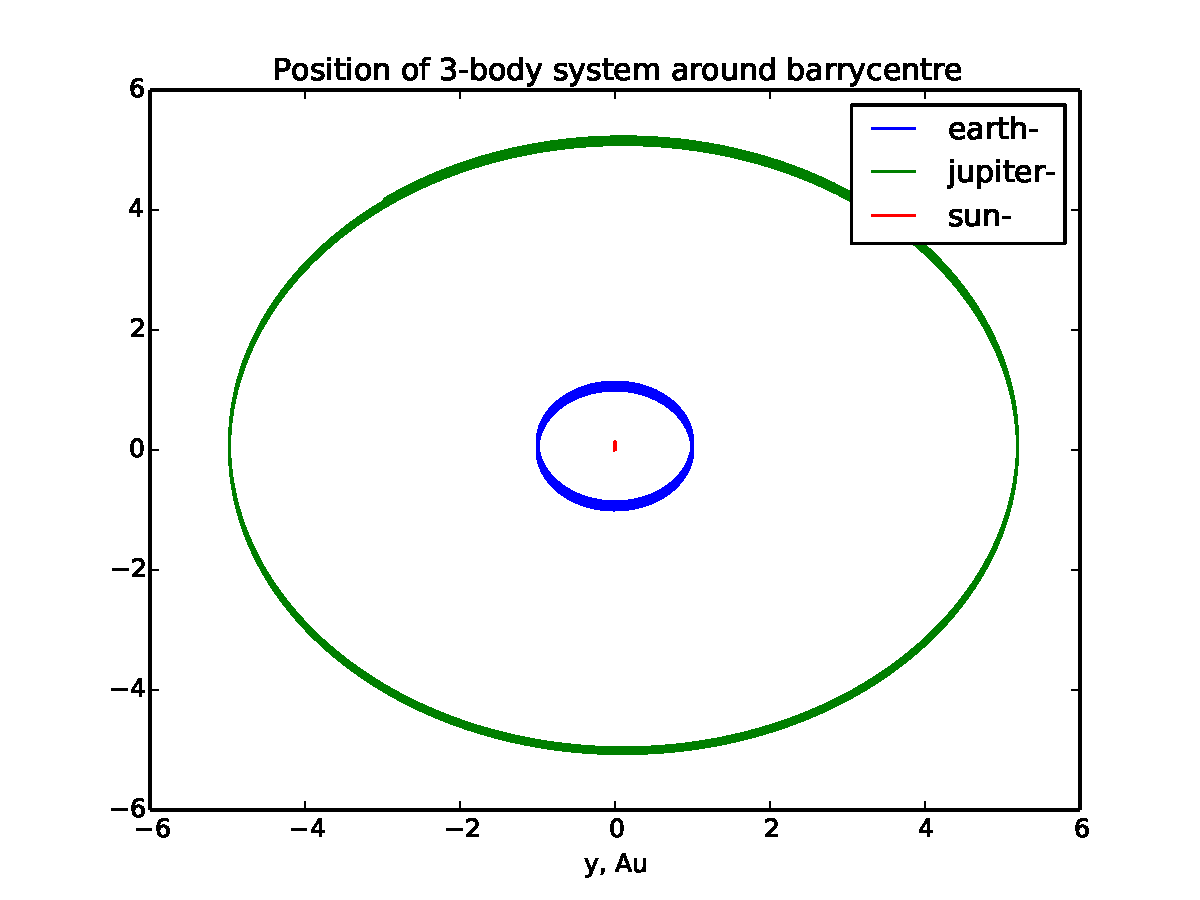
\includegraphics[width=0.9\linewidth]{../results/plots/3bodyCentric_position}
	\caption{}
	\label{fig:3bodycentricposition}
\end{figure}

\begin{figure}
	\centering
	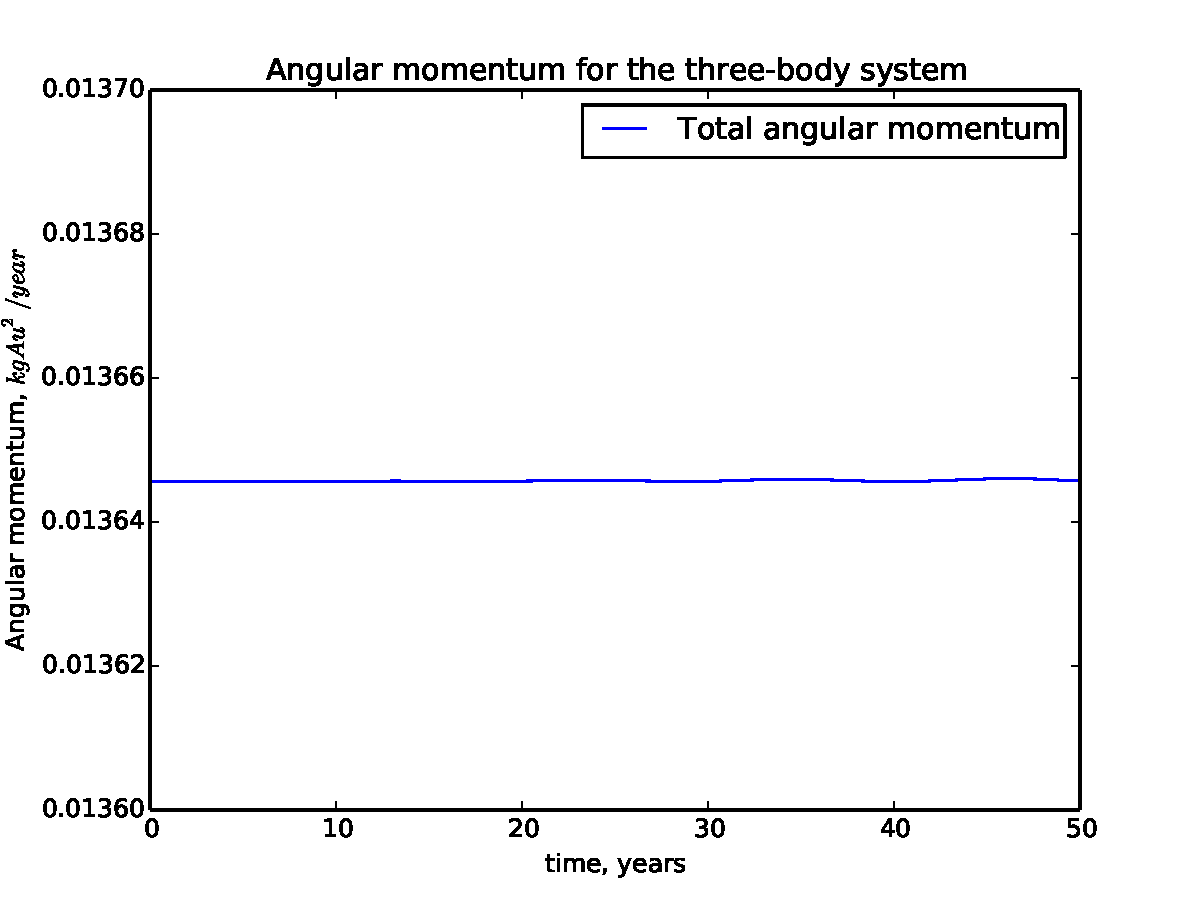
\includegraphics[width=0.9\linewidth]{../results/plots/3bodyCentric_angular}
	\caption{}
	\label{fig:3bodycentricangular}
\end{figure}

\begin{figure}
	\centering
	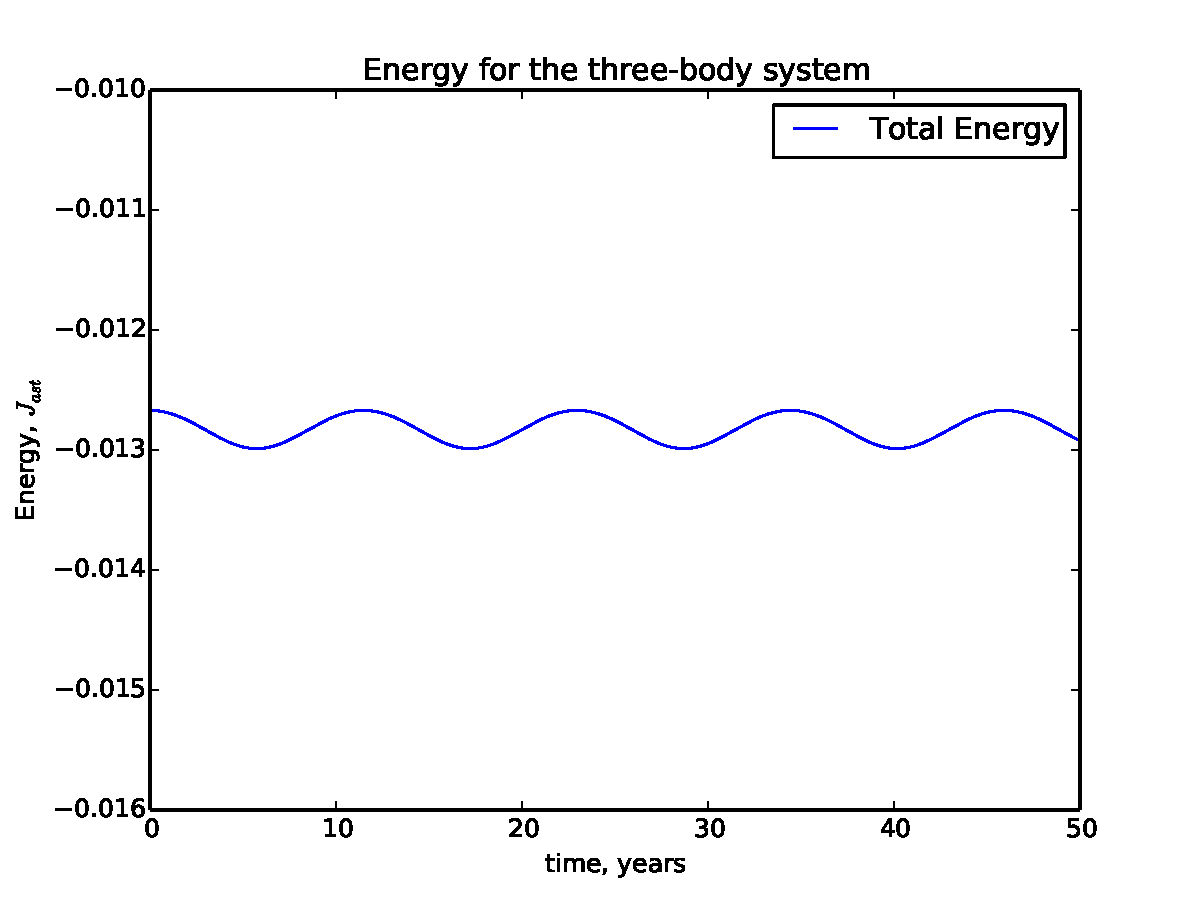
\includegraphics[width=0.9\linewidth]{../results/plots/3bodyCentric_energy}
	\caption{}
	\label{fig:3bodycentricenergy}
\end{figure}


	Ok - if initial values are correct.
	
	- Plot Earth's motion for increased mass of Jupiter (3 masses)

	same.	
	
	- Find center off mass - use as origin

	Found and incorporated.	
	
	- Give sun initial velocity so momentum is zero (origin is fixed)

	How? What momentum? velocity?	
	
	- Compare with 3e)
	- Extend to all planets (plot)
	
	
\subsection{All planets}

At last we added all the planets with initial conditions form NASA \cite{nasa}. Figure \ref{fig:solarsystem_allplanets} shows the orbits of all the planets and Figure \ref{fig:solarsystem_innerplanets} shows the inner planet's orbits, because they are difficult to distinguish in the other plot.  

\begin{figure}[H]
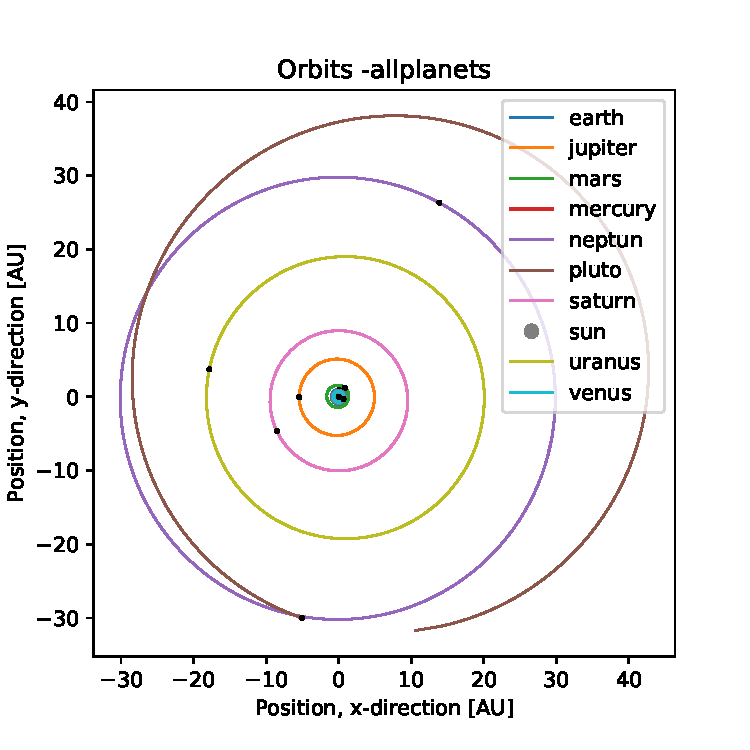
\includegraphics[width=1\linewidth]{../results/plots/plotof-earthjupiter-allplanets.pdf}\caption{This is a plot of the Solar System after 100 years of motion.}\label{fig:solarsystem_allplanets}
\end{figure}


\begin{figure}[H]
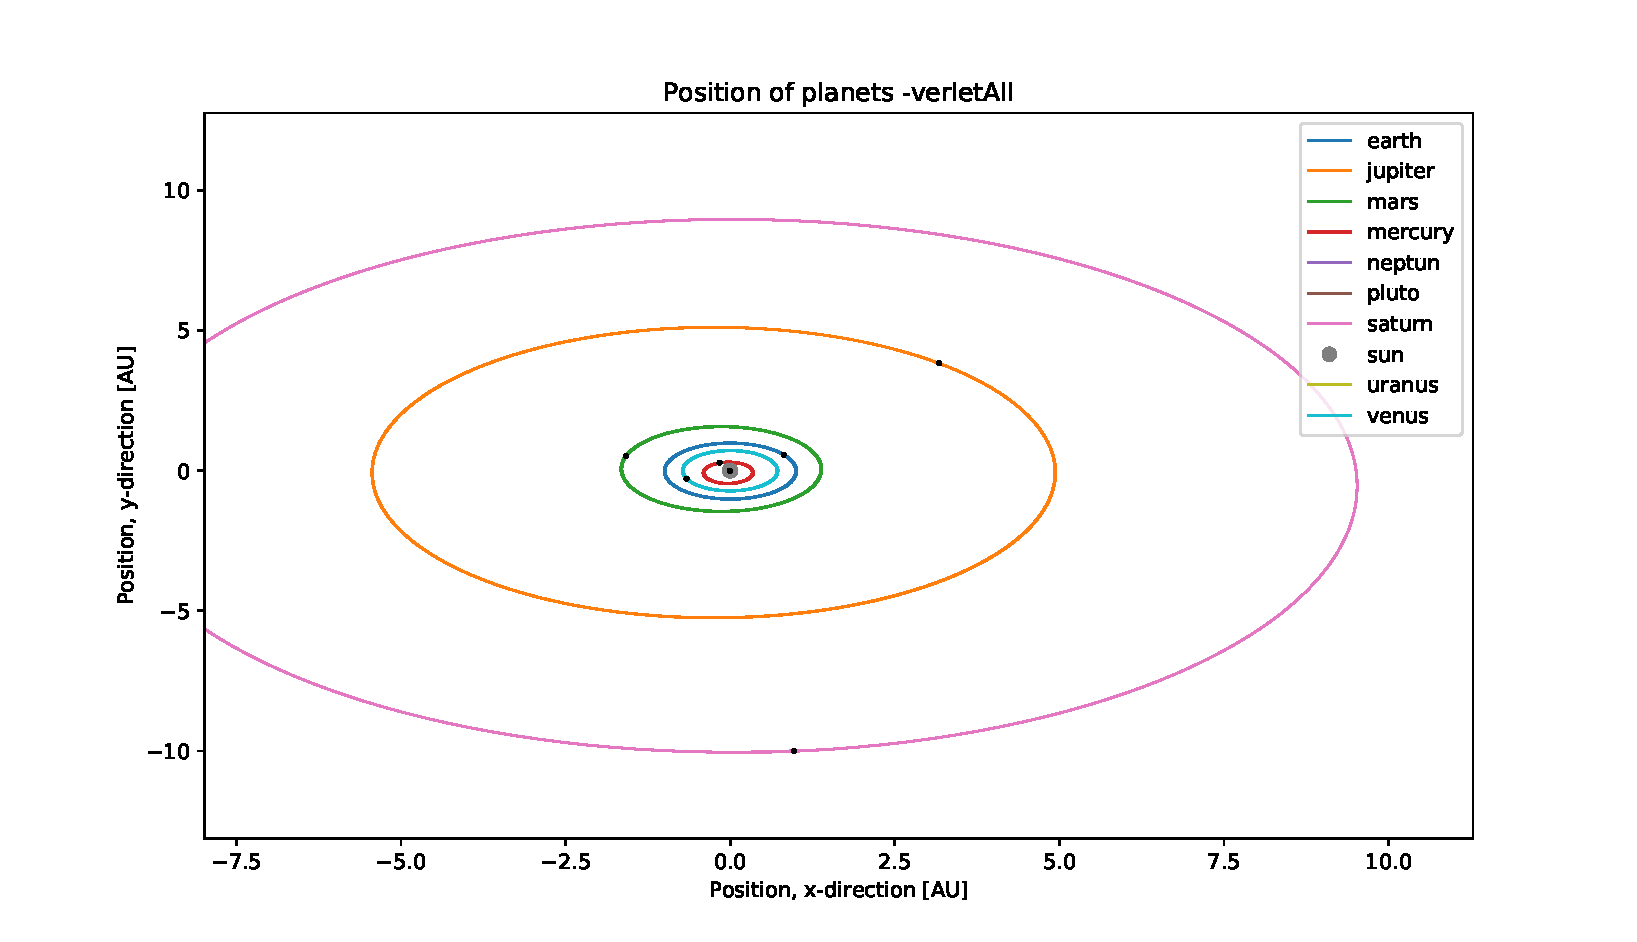
\includegraphics[width=1\linewidth]{../results/plots/innerplanets-verletAll.pdf}\caption{This is a plot of planets closest to the sun in the Solar System after 30 years of motion.}\label{fig:solarsystem_innerplanets}
\end{figure}
	
\subsection{Considering relativistic force}
	
As a last point we wanted to see how relativistic forces affect the orbits. We used the perihelion precession of Mercury to explore this. Table \ref{tab:Perihelion} shows the perihelion position of Mercury after 100 years of orbiting the sun alone with no other planets affecting the movement. The table lists the position with non-relativistic forces and relativistic forces.
	
\begin{table}[H]\caption{This is a table with the Perihelion information about Mercury after one century, 100 years. The perihelion precession is observed to be 43 arc seconds and, as we can see, this fits well with our result.}\label{tab:Perihelion}
  \begin{tabular}{lll} 
    & Position [AU] & Angle [arcs]\\ \hline 
    Initial values: &($0.3075,  0$)& $ 0$\\ 
    Newtonian &($0.3075,  -1.519\E{-7} $)& $  -0.102 $\\ 
    Relativistic & ($ 0.3075, 6.447\E{-5} $)  &$ 43.247 $ \\ 
\end{tabular}
\end{table}
